% Generated by fikzPy
\documentclass[tikz,border=0pt]{standalone}
\usepackage{tikz}

\begin{document}
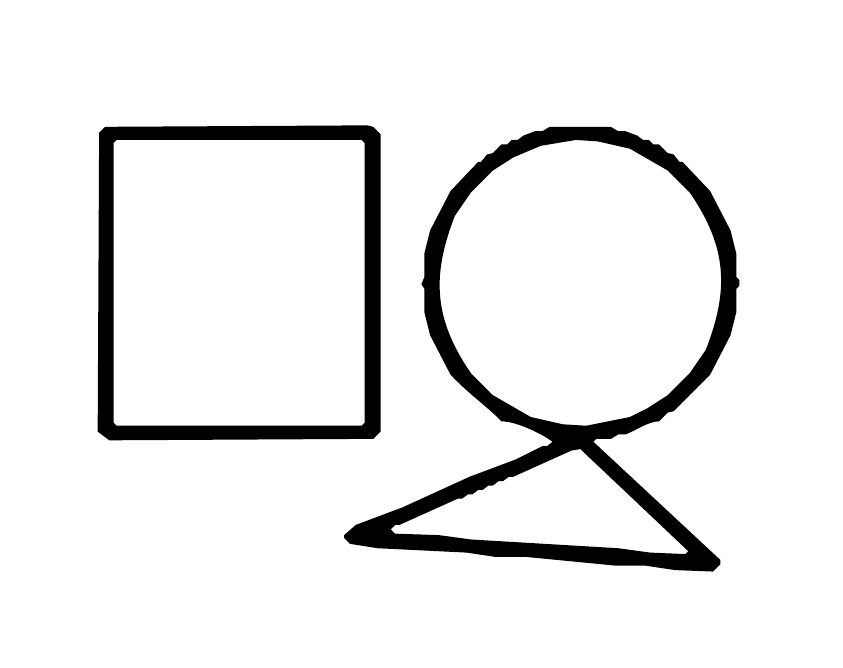
\begin{tikzpicture}[scale=1]
  \begin{scope}
  \clip (0,0) rectangle (10.0,7.777777777777778);

  \draw[draw=none,fill=black,even odd rule] (8.3148, 6.0741) -- (8.2778, 6.0741) -- (8.2037, 6.1667) -- (8.1296, 6.1852) -- (8.0185, 6.2963) -- (7.9444, 6.2963) -- (7.8889, 6.3518) -- (7.8148, 6.3518) -- (7.7407, 6.4074) -- (7.5926, 6.4629) -- (7.5, 6.4629) -- (7.4074, 6.5185) -- (6.6296, 6.5185) -- (6.5371, 6.4629) -- (6.4444, 6.4629) -- (6.2963, 6.4074) -- (6.2222, 6.3518) -- (6.1482, 6.3518) -- (6.0926, 6.2963) -- (6.0185, 6.2963) -- (5.9074, 6.1852) -- (5.8333, 6.1667) -- (5.7593, 6.0741) -- (5.7222, 6.0741) -- (5.3704, 5.7037) -- (5.1111, 5.2037) -- (5.0371, 4.9074) -- (5.0371, 4.6111) -- (5.0, 4.5185) -- (5.0371, 4.4629) -- (5.0371, 4.1667) -- (5.1111, 3.8704) -- (5.3704, 3.3704).. controls (5.6175, 3.1102) and (5.7953, 3.001) .. (6.0185, 2.7778).. controls (6.2029, 2.7778) and (6.5109, 2.6298) .. (6.6667, 2.5185) -- (6.5926, 2.4629) -- (6.5371, 2.4629) -- (6.2037, 2.2963) -- (5.6111, 2.0741) -- (4.7593, 1.6852) -- (4.1667, 1.4629) -- (4.0185, 1.3333) -- (4.0185, 1.2963) -- (4.0926, 1.2222) -- (4.4444, 1.1667) -- (5.5741, 1.1111) -- (5.9444, 1.0556) -- (6.3333, 1.0556) -- (7.4815, 0.9444) -- (7.8518, 0.9444) -- (8.2222, 0.8889) -- (8.7037, 0.8704) -- (8.7963, 0.9629) -- (8.7963, 1.0185) -- (7.1852, 2.5185) -- (7.2222, 2.5556) -- (7.4074, 2.5556) -- (7.5, 2.6111) -- (7.5926, 2.6111).. controls (7.7306, 2.6629) and (7.8816, 2.7778) .. (8.0185, 2.7778) -- (8.1296, 2.8889) -- (8.2037, 2.9074) -- (8.6667, 3.3704) -- (8.9259, 3.8704) -- (9.0, 4.1667) -- (9.0, 4.4629) -- (9.0371, 4.5) -- (9.0371, 4.5741) -- (9.0, 4.6111) -- (9.0, 4.9074) -- (8.9259, 5.2037) -- (8.6667, 5.7037) -- (8.3148, 6.0741) -- cycle (0.9815, 6.5185) -- (0.9074, 6.4444) -- (0.8889, 2.6482) -- (1.0371, 2.5371) -- (4.3889, 2.5556) -- (4.4815, 2.6482) -- (4.4815, 6.4259) -- (4.3889, 6.5185) -- (4.3148, 6.5371) -- (0.9815, 6.5185) -- cycle (1.1296, 6.3518) -- (4.2407, 6.3518) -- (4.2778, 6.3148) -- (4.2778, 2.7593) -- (4.2407, 2.7222) -- (1.1296, 2.7222) -- (1.0926, 2.7593) -- (1.0926, 6.3148) -- (1.1296, 6.3518) -- cycle (6.9629, 6.3518) -- (7.2407, 6.3333) -- (7.6482, 6.2407) -- (8.1296, 5.9629) -- (8.4074, 5.6852).. controls (8.8883, 4.9857) and (8.9069, 4.4412) .. (8.6111, 3.6852) -- (8.4074, 3.3889) -- (8.1296, 3.1111) -- (7.8704, 2.9444) -- (7.6482, 2.8333) -- (7.0926, 2.7222) -- (6.7963, 2.7407) -- (6.3889, 2.8333) -- (5.9074, 3.1111) -- (5.6296, 3.3889).. controls (5.1528, 4.0825) and (5.1302, 4.6331) .. (5.4259, 5.3889) -- (5.6296, 5.6852) -- (5.9074, 5.9629) -- (6.1667, 6.1296) -- (6.5185, 6.2778) -- (6.9629, 6.3518) -- cycle (8.3889, 1.1296) -- (8.3518, 1.0926) -- (7.9074, 1.1111) -- (7.5, 1.1667) -- (5.6296, 1.2778) -- (5.2222, 1.3333) -- (4.6667, 1.3518) -- (4.6111, 1.4074) -- (4.6667, 1.4629) -- (4.7222, 1.4629) -- (5.4629, 1.7963) -- (5.5185, 1.7963) -- (5.5926, 1.8518) -- (5.6482, 1.8518) -- (5.7222, 1.9074) -- (5.7778, 1.9074) -- (5.8518, 1.9629) -- (5.9074, 1.9629) -- (5.9815, 2.0185) -- (6.0371, 2.0185) -- (6.1111, 2.0741) -- (6.1667, 2.0741) -- (6.9074, 2.4074) -- (7.0185, 2.4259) -- (8.3889, 1.1296) -- cycle;




\end{scope}
\pgfresetboundingbox
\path[use as bounding box] (0,0) rectangle (10.0,7.777777777777778);
\end{tikzpicture}
\end{document}
